\chapter{Análisis Operacional y Flujo}
\noindent
\section{Teoría previa}
\subsection{Estación de servicio}
\begin{multicols}{2}
\begin{figure}[H]
    \centering
    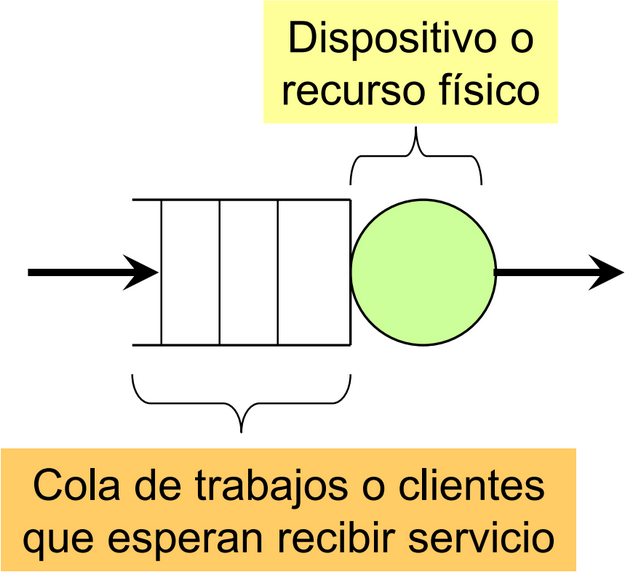
\includegraphics[width=0.5\textwidth]{Images/Estacion_ser.png}
    \caption{Estación de servicio}
\end{figure}
\begin{figure}[H]
    \centering
    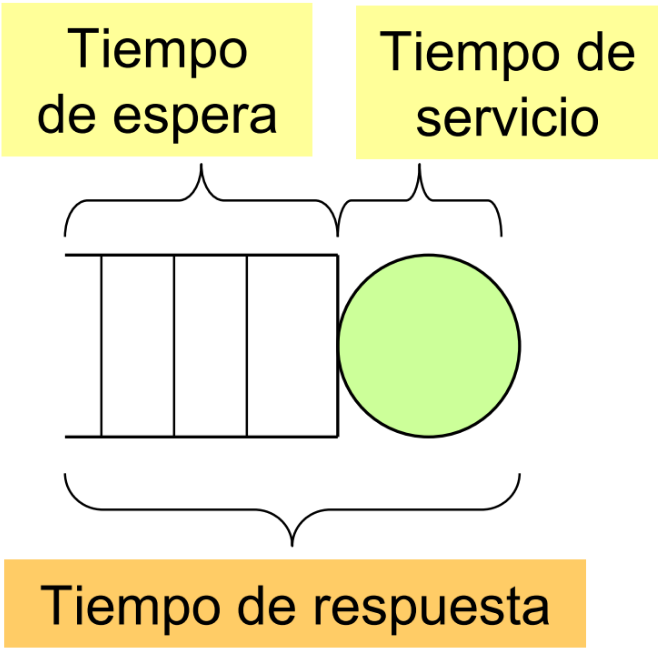
\includegraphics[width=0.43\textwidth]{Images/tiempos_est.png}
    \caption{Tiempos}
\end{figure}
\end{multicols}
Una \textbf{estación de servicio} es un objeto abstracto compuesto por un servidor y una cola de espera. En ella los trabajos o tareas entrantes ($A$) hacen cola ordenadamente para ser procesadas y transformadas en tareas de salida ($C$).\\

Por ejemplo una impresora puede tener varios trabajos para imprimir en cola, que de forma ordenada va transformando en impresiones en papel.
\newpage
\subsection{Nomenclatura y variables}
\begin{itemize}
    \item $A$: tareas entrantes.
    \item $C$: tareas salientes.
    \item $B$: tiempo ocupado (busy).
    \item $T$: tiempo de medición.
    \item $\lambda$: tasa de llegadas.
    \item $X$: productividad.
    \item $U$: utilización.
    \item $S$: tiempo de servicio / ejecución.
    \item $V$: número de accesos.
    \item $R$: tiempo de respuesta / acceso.
    \item $W$: tiempo de espera (wating).
    \item $N$: número de trabajos (en cola y en servicio) en una estación.
    \item $Q$: número de trabajos en espera (queued).
    \item $D$: demandas de servicio.
    \item $Z$: Tiempo de reflexión.
    \item \textbf{HFE}: Hipótesis de flujo equilibrado.
\end{itemize}
\subsection{Fórmulas y leyes}
\begin{multicols}{2}
\[\lambda = \dfrac{A}{T}[t/s]\]
\[X = \dfrac{C}{T} = \dfrac{1}{D}[t/s]\]
\[E_{rel}= \dfrac{|A-C|}{C}\]
\[E_{abs}=|A-C|\]
\[U = \dfrac{B}{T}=X\cdot S[s]\]
\[S = \dfrac{U}{X}[s/t]\]
\[S = \dfrac{B}{C}[s/t]\]
\[S=T_{posic}+T_{latencia}+T_{transf}[s/t]\]
\[R = \dfrac{B}{T}[s]\]
\[R= \dfrac{1}{n}\sum_{i=1}^{n}R_i[s]\]
\[R = \sum_{i=1}^{n}V_i\cdot R_i = \sum_{i=1}^{n}D_i[s]\]
\[R = \sum_{i=1}^{n}C_i-A_i[s]\]
\[W = R-S[s]\]
\[X(N)\leq min(\dfrac{N}{D+Z}, \dfrac{1}{D_b})\]
\[D=V\cdot S\]
\[R(N)\geq max(D, N\cdot D_b-Z)\]
\end{multicols}

\subsubsection{Hipótesis de flujo equilibrado}
    La Hipótesis de flujo equilibrado lo que supone es que la cantidad de tareas entantes es igual a la cantidad de tareas salientes: $A = C$.\\
    Esto implica que la tasa de llegadas coincide con la productividad: $\lambda = X$
\subsubsection{Error cuadrático medio}
    Cuando queremos calcular el error que supone asumir HFE con respecto a \textbf{varios periodos} de medición ($n$) debemos usar el error cuadrático medio. \[ECM = \dfrac{1}{n}\sum_{i=1}^{n}(A_i - C_i)^2 \]
\subsubsection{Ley de Little}
    Relaciona el número de trabajos en el sistema con el tiempo de permanencia y su productividad o tasa de llegada.\\
    \[N = \lambda \cdot R = X\cdot R\]\\
    La ley de little también se puede aplicar a programas en cola:\\
    \[N = \lambda \cdot W = X\cdot W\]
\subsubsection{Ley de flujo forzado}
   Establece que el flujo a través de un determinado dispositivo determina el flujo en cualquier otro dispositivo. La ley es válida solo si también lo es la HFE.
   \[X = V_i \cdot X_0\]
   donde $X$ es la productividad del sistema, $X_0$ es la productividad del dispositivo y $V_i$ es la razón de visitas al dispositivo.
   
\subsubsection{Cuello de botella}
    En el contexto de esta asignatura llamaremos cuello de botella al dispositivo de un sistema que posea mayor demanda ($D$).
%%%%%%%%%%%%%%%%%%%%%%%%%%%%%%%%%%%%%%%%%%%%%%%%%%%%%%%%%%%
\newpage
\section{Ejercicios resueltos}
Los ejercicios del 1 al 8 son de sistemas interactivos y los ejercicios del 9 al 12 son sobre sistemas transaccionales, siendo los dos últimos sobre grafos.

\subsection{Ejercicio 1}
El disco de un computador se ha monitorizado durante un periodo de 30 segundos. Durante este tiempo
han llegado 11 peticiones y han acabado 12. Se sabe que el disco ha estado vacío durante 2.5 segundos y
se ha podido medir el tiempo de respuesta de 9 peticiones. Estos tiempos, expresados en segundos, son:\\
8.2, 9.1, 2.3, 5.9, 2.0, 6.2, 4.1, 6.5, 7.3. \\Se pide calcular:
\begin{enumerate}
    \item La exactitud con que se cumple la \textbf{hipótesis del flujo equilibrado} de trabajos de acuerdo a los datos. ¿Cómo se calcularía si se hubieran monitorizado 10 periodos de 30 segundos?
        \begin{tcolorbox}[colback=white,colframe=cyan!50!black,fonttitle=\bfseries]
        Lo que nos estan pidiendo es el error que tienen los resultados obtenidos con respecto a \textbf{HFE}.\\
        Existen dos tipos de errores:
        \begin{itemize}
            \item \textbf{Error relativo}: normalmente lo calcularemos siempre con respecto a la salida (dividimos por $C_i$):\\ $E_r=\dfrac{|A_i - C_i|}{C_i}=\dfrac{1}{12}=0.083$\\
            El error relativo es del 8,3\%
            \item \textbf{Error absoluto}: $E_a=|A_i-C_i|=1$
        \end{itemize}
        Para los casos en los que queremos medir varios periodos debemos recurrir al \textbf{error cuadrático medio}. $ECM = \dfrac{1}{n}\sum_{i=1}^{n}(A_i - C_i)^2 = \dfrac{1}{10}\sum_{i=1}^{10}(A_i - C_i)^2$
        \end{tcolorbox}
    \item La tasa de llegadas de peticiones al disco y el tiempo entre llegadas.
    \begin{tcolorbox}[colback=white,colframe=cyan!50!black,fonttitle=\bfseries]
$\lambda = \dfrac{A}{T}=\dfrac{11}{30}=0.367[t/s]$; T entre llegadas $ = \dfrac{1}{\lambda}=\dfrac{30}{11}=2.73[s]$
    \end{tcolorbox}
    \item La productividad del disco.
    \begin{tcolorbox}[colback=white,colframe=cyan!50!black,fonttitle=\bfseries]
$X = \dfrac{C}{T}=\dfrac{12}{30}=0.4[t/s]$
    \end{tcolorbox}
    \item La utilización del disco.
    \begin{tcolorbox}[colback=white,colframe=cyan!50!black,fonttitle=\bfseries]
    En este caso, el tiempo de ocupación lo obtenemos de restar el tiempo de medición menos el tiempo que ha estado vacío:\\ $B = T-T_{vacio} = 30-2.5=27.5$\\\\
    $U = \dfrac{B}{T}=\dfrac{27.5}{30}=0.917=91.7\%$
    \end{tcolorbox}
    \item El tiempo medio de servicio del disco.
    \begin{tcolorbox}[colback=white,colframe=cyan!50!black,fonttitle=\bfseries]
$S = \dfrac{U}{X}=\dfrac{0.917}{0.4}=2.29[s/t]$
    \end{tcolorbox}
    \item El tiempo medio de espera en cola.
    \begin{tcolorbox}[colback=white,colframe=cyan!50!black,fonttitle=\bfseries]
    Primero calculamos el tiempo de respuesta con la fórmula del sumatorio.\\
    $R = \dfrac{1}{n}\sum_{i=1}^{n}R_i = \dfrac{1}{9}\sum_{i=1}^{9}R_i=5.73[s]$\\
    Y sustituimos\\
    $W = R-S = 5.73-2.29=3.44[s]$
    \end{tcolorbox}
\end{enumerate}

%%%%%%%%%%%%%%%%%%%%
\subsection{Ejercicio 2}
En un sistema cliente-servidor se considera que las transacciones usan 4ms de procesador en el cliente, 6ms de procesador en el servidor y cada transacción visita la unidad de disco un total de 12 veces, es decir, se leen 12 bloques (de 1024 bytes) del disco del servidor. De las características técnicas del disco se sabe que el tiempo medio de posicionamiento es de 8ms, la latencia media es 3.6ms y el tiempo de transferencia es  $42.66 x 10^{-6}$ segundos. Se pide:
\begin{enumerate}
    \item El tiempo de servicio de las transacciones en los procesadores del cliente y del servidor, expresadas en segundos.
    \begin{tcolorbox}[colback=white,colframe=cyan!50!black,fonttitle=\bfseries]
    De los datos del enunciado podemos sacar la siguiente tabla que representa una transacción:
    \begin{table}[H]\centering\begin{tabular}{|c|c|c|}\hline
    \textbf{Dispositivo}    & \textbf{Vi} & \textbf{Si(ms)} \\ \hline
    Cliente & \multirow{2}{*}{12}& 4  \\ \cline{1-1} \cline{3-3}
    Servidor && 6   \\ \hline
    \end{tabular}\end{table}
    Como nos piden $S$ en segundos, simplemente tenemos que convertir:\\
    $S_{cliente}=4\cdot10^{-3}[s]$;  $S_{servidor}=6\cdot10^{-3}[s]$
    \end{tcolorbox}
    \item El tiempo de servicio S del disco en un caso general, es decir teniendo en cuenta el tiempo de posicionamiento, la latencia y el tiempo de transferencia.
    \begin{tcolorbox}[colback=white,colframe=cyan!50!black,fonttitle=\bfseries]
$S =T_{posic}+T_{latencia}+T_{transf}=8\cdot10^{-3}+3.6\cdot10^{-3}+0.04266\cdot10^{-3}=11.64266\cdot10^{-3}[s]$
    \end{tcolorbox}
    \item El tiempo de una transacción suponiendo dos casos: que los bloques estén grabados en pistas diferentes (peor caso) o situados de forma consecutiva (mejor caso).
    \begin{tcolorbox}[colback=white,colframe=cyan!50!black,fonttitle=\bfseries]
    En todas las transacciones debemos de tener en cuenta el tiempo de transferencia.\\
    En el \textbf{caso peor} todas las transacciones implican posicionamiento y latencia, por tanto:\\
    $12\cdot S=12\cdot11.64266\cdot10^{-3}=139.7119\cdot10^{-3}[s]$\\
    En el \textbf{caso mejor} solo deberá posicionarse en el primer acceso, por tanto:\\
    $12\cdot T_{transf}+(T_{posic}+T_{latencia})=12\cdot0.04266\cdot10^{-3}+(8\cdot10^{-3}+3.6\cdot10^{-3})[s]$
    \end{tcolorbox}
    \item ¿Qué componentes del tiempo de servicio del disco influyen más en el rendimiento? ¿Por qué son importantes las operaciones de compactificación de discos?
    \begin{tcolorbox}[colback=white,colframe=cyan!50!black,fonttitle=\bfseries]
    Los componentes que más influyen son el tiempo de posicionamiento y el tiempo de latencia.\\Para reducir los tiempos de acceso a la información.
    \end{tcolorbox}
\end{enumerate}

%%%%%%%%%%%%%%%%%%%%
\subsection{Ejercicio 3}
Durante una sesión de medida de media hora, un monitor software ha extraído las siguientes variables operacionales básicas de un servidor web:

\begin{table}[H]\centering
\begin{tabular}{|c|c|}
\hline
\textbf{Variable} & \textbf{Valor}          \\ \hline
A        & 364 peticiones \\ \hline
C        & 359 peticiones \\ \hline
B        & 23 minutos     \\ \hline
\end{tabular}
\end{table}
Calcula las siguientes variables operacionales deducidas del servidor web: tasa de llegadas, productividad, utilización y tiempo medio de servicio.
\begin{tcolorbox}[colback=white,colframe=cyan!50!black,fonttitle=\bfseries]
$\lambda = \dfrac{A}{T} = \dfrac{364}{30\cdot60}=0.202[t/s]$; 
$X = \dfrac{C}{T}=\dfrac{359}{30\cdot60}=0.199[t/s]$\\\\
$U = \dfrac{B}{T}=\dfrac{23\cdot60}{30\cdot60}=0.766[s]$; 
$S = \dfrac{U}{X}=\dfrac{0.766}{0.199}=3.844[s/t]$
\end{tcolorbox}
%%%%%%%%%%%%%%%%%%%%
\subsection{Ejercicio 4}
Un procesador recibe una media de 5 programas por segundo. Cada programa experimenta un tiempo medio de ejecución de 0.14 segundos y un tiempo medio de respuesta de 8 segundos. Se pide:
\begin{itemize}
    \item Uso medio del procesador.
    \begin{tcolorbox}[colback=white,colframe=cyan!50!black,fonttitle=\bfseries]
    El enunciado nos dice que: $S=0.14[s]$; $A=5[t]$; $R=8[s]$\\
    Sabemos que: \\
    $S =\dfrac{U}{X}$;  $X = \dfrac{C}{T}$; $\lambda = \dfrac{A}{T}$\\
    Como no tenemos $C$, podemos asumir \textbf{HFE}, por tanto:\\
    $S =\dfrac{U}{\lambda}$, y calculamos:\\\\
    $\lambda = \dfrac{A}{T} = \dfrac{5}{1} = 5[t]$ al ser una media, ponemos $T=1$\\\\
    $S =\dfrac{U}{\lambda}$; $U = S \cdot \lambda = 0.14\cdot5=0.7=70[\%]$ 
    \end{tcolorbox}
    \item Tiempo medio de espera en la cola del procesador.
    \begin{tcolorbox}[colback=white,colframe=cyan!50!black,fonttitle=\bfseries]
    $W = R-S= 8-0.14 = 7.86[s]$
    \end{tcolorbox}
    \item Número medio de programas en la cola de espera del procesador.
    \begin{tcolorbox}[colback=white,colframe=cyan!50!black,fonttitle=\bfseries]
    Aplicamos la ley de little:
    $N=X\cdot W=5\cdot7.86=39.3[t]$
    \end{tcolorbox}
\end{itemize}

%%%%%%%%%%%%%%%%%%%%
\subsection{Ejercicio 5}
Después de monitorizar el procesador de un servidor web durante un periodo de 30 segundos, se sabe que ha sido utilizado durante 27 segundos. También se han contabilizado 74 llegadas y 72 salidas de peticiones. Se pide:
\begin{enumerate}
    \item Porcentaje de error cometido al asumir la hipótesis del flujo equilibrado.
    \begin{tcolorbox}[colback=white,colframe=cyan!50!black,fonttitle=\bfseries]
    Calculamos el error relativo: $E_r=\dfrac{|A_i - C_i|}{C_i}=\dfrac{2}{72}=0.027=2.7[\%]$\\
    \end{tcolorbox}
    \item Tasa de llegadas al procesador.
    \begin{tcolorbox}[colback=white,colframe=cyan!50!black,fonttitle=\bfseries]
    $\lambda = \dfrac{A}{T} = \dfrac{74}{30} = 2.46 [t/s]$
    \end{tcolorbox}
    \item Utilización del procesador.
    \begin{tcolorbox}[colback=white,colframe=cyan!50!black,fonttitle=\bfseries]
    $U = \dfrac{B}{T} = \dfrac{27}{30} = 0.9[s] = 90[\%]$
    \end{tcolorbox}
    \item Si cada trabajo realiza una media de cuatro visitas al procesador, ¿cuál es la productividad del servidor web?
    \begin{tcolorbox}[colback=white,colframe=cyan!50!black,fonttitle=\bfseries]
    Para hallar la productividad de un dispositivo del sistema debemos aplicar la ley de flujo forzado:
    $X_i = V_i \cdot X_0$\\ Por tanto $X_0 = \dfrac{X}{V_i} = \dfrac{2.46}{4} = 0.6$
    \end{tcolorbox}
    \item Se han monitorizado 3 periodos adicionales de 30” y se han obtenido los siguientes datos:
    \begin{itemize}
        \item Llegadas: 74, 75, 77
        \item Salidas: 73, 72, 70
        \item Busy: 29, 26, 25
    \end{itemize}
    Calcular el ECM de la hipótesis del flujo equilibrado, y los resultados de los apartados b-d para estos nuevos datos.
    \begin{tcolorbox}[colback=white,colframe=cyan!50!black,fonttitle=\bfseries]
    $ECM = \dfrac{1}{n}\sum_{i=1}^{n}(A_i - C_i)^2 = \dfrac{1}{4}\cdot(2^2 + 1^2 + 3^2 + 7^2) = \dfrac{63}{4}=15.75$
    \begin{itemize}
        \item $\lambda = \dfrac{300}{120} = 2.5[t/s]$
        \item $U = \dfrac{107}{120} = 0.89=89[\%]$
        \item $X_0 = \dfrac{X}{V_i} = \dfrac{2.5}{4} = 0.625$
    \end{itemize}
    \end{tcolorbox}
\end{enumerate}


%%%%%%%%%%%%%%%%%%%%
\subsection{Ejercicio 6}

Tenemos una unidad de disco duro cuya controladora dispone de cierta cantidad de memoria caché. El tiempo medio de acceso a la controladora es de 0.1ms, el tiempo medio de posicionamiento del disco es de 5ms, la latencia rotacional media es de 6ms y el tiempo medio de transferencia es de 0.3ms.\\

Sabiendo que la memoria caché tiene una probabilidad de acierto del 95\%, se pide determinar el tiempo medio de servicio de la unidad de disco. Ídem en el caso de que la probabilidad de acierto sea del 98\%, 80\% y del 70\%.\\
\begin{tcolorbox}[colback=white,colframe=cyan!50!black,fonttitle=\bfseries]
Para $P=0.95$: $S = 0.1+(5+6+0.3)\cdot0.05=0.665[ms]$\\
Para $P=0.98$: $S = 0.1+(5+6+0.3)\cdot0.02=0.326[ms]$\\
Para $P=0.80$: $S = 0.1+(5+6+0.3)\cdot0.2=2.36[ms]$\\
Para $P=0.70$: $S = 0.1+(5+6+0.3)\cdot0.3=3.49[ms]$
\end{tcolorbox}
%%%%%%%%%%%%%%%%%%%%
\subsection{Ejercicio 7}

Considera un modelo cerrado de sistema informático con los siguientes parámetros:
\begin{table}[H]\centering
\begin{tabular}{|c|c|c|}
\hline
\textbf{Dispositivo} & \textbf{Vi} & \textbf{Ri(ms)} \\ \hline
Procesador  & 7  & 4,3    \\ \hline
Disco 1     & 2  & 1,5    \\ \hline
Disco 2     & 4  & 2,3    \\ \hline
\end{tabular}
\end{table}
Determina el tiempo medio de respuesta de una petición a este sistema informático. Si el número medio de peticiones activas en el sistema es 80, ¿cuál es la tasa de llegadas que soporta?
\begin{tcolorbox}[colback=white,colframe=cyan!50!black,fonttitle=\bfseries]
Tiempo medio de respuesta $R=\sum_{i=1}^{3}V_i\cdot R_i=42.3[ms]$\\\\
Ley de little: $N = \lambda \cdot R$; $\lambda = \dfrac{N}{R}=\dfrac{80}{0.0423}=1891.25[t/s]$
\end{tcolorbox}
%%%%%%%%%%%%%%%%%%%%
\subsection{Ejercicio 8}
Durante un periodo de medida de 5 segundos se ha obtenido la siguiente información sobre los instantes de llegada y de salida de peticiones a un disco:
\begin{table}[H]\centering
\begin{tabular}{|c|c|c|c|c|c|c|c|c|c|c|}
\hline
\textbf{Petición} & 1    & 2    & 3    & 4    & 5    & 6    & 7    & 8    & 9    & 10   \\ \hline
\textbf{Llegada}  & -    & -    & -    & 0.34 & 1.76 & 2.21 & 3.84 & 4.39 & 4.77 & 4.90 \\ \hline
\textbf{Salida}   & 0.98 & 1.82 & 2.10 & 2.58 & 2.95 & 3.12 & 4.24 & 4.66 & -    & -    \\ \hline
\end{tabular}
\end{table}
\begin{enumerate}
    \item ¿Con qué precisión se cumple la ley del flujo equilibrado?
    \begin{tcolorbox}[colback=white,colframe=cyan!50!black,fonttitle=\bfseries]
    $E_r=\dfrac{|A-C|}{C}=\dfrac{|7-8|}{8}=0.125=12.5[\%]$
    \end{tcolorbox}
    \item ¿Cuál es la productividad y el tiempo medio de respuesta del disco?
    \begin{tcolorbox}[colback=white,colframe=cyan!50!black,fonttitle=\bfseries]
    $X=\dfrac{C}{T}=\dfrac{8}{5}=1.6[t/s]$\\
    En este caso, para calcular $R$, debemos quedarnos con las peticiones de las que conocemos todos sus datos (en este caso 4, 5, 6, 7 y 8), que son 5 peticiones.
    $R=\dfrac{1}{5}\cdot \sum_{i=4}^{8}C_i-A_i = 1.002[s]$
    \end{tcolorbox}
    \item ¿Cuántas peticiones soporta de media el disco?
    \begin{tcolorbox}[colback=white,colframe=cyan!50!black,fonttitle=\bfseries]
    Ley de little: $N=X\cdot R=1.6\cdot1.002=1.6032 [t]$
    \end{tcolorbox}
    \item ¿Cuál es la utilización y el tiempo de servicio del disco?
    \begin{tcolorbox}[colback=white,colframe=cyan!50!black,fonttitle=\bfseries]
    Recordemos que: $S=\dfrac{B}{C}$\\
    Para obtener el tiempo ocupado ($B$) restamos el tiempo total de medición ($T$) menos el tiempo en el que no se ha estado ejecutando nada, de manera que:\\
    $B=5 - ((4.77-4.66) + (4.39-4.24) + (3.84-3.12)) = 4.02 [s]$\\
    Entonces: $S=\dfrac{4.02}{8} = 0.5025[s]$
    \end{tcolorbox}
\end{enumerate}

%%%%%%%%%%%%%%%%%%%%
\subsection{Ejercicio 9}
Considera un modelo abierto de sistema informático con los siguientes parámetros:
\begin{table}[H]\centering\begin{tabular}{|c|c|c|}\hline
\textbf{Dispositivo}    & \textbf{Vi} & \textbf{Si[s]} \\ \hline
Procesador (1) & 17 & 0.03   \\ \hline
Disco 2        & 6  & 0,04   \\ \hline
Disco 3        & 10 & 0,04   \\ \hline
\end{tabular}\end{table}
El tiempo medio entre llegadas de clientes es de 0,6 segundos. Se pide calcular:
\begin{enumerate}
    \item La tasa de llegadas al sistema.
    \begin{tcolorbox}[colback=white,colframe=cyan!50!black,fonttitle=\bfseries]
    Al tratarse de tiempo medio, usamos 1 como valor de $A$:\\
    $\lambda = \dfrac{A}{C} = \dfrac{1}{0.6} = 1.66[t/s]$
    \end{tcolorbox}
    \item Las demandas de servicio de los dispositivos.
    \begin{tcolorbox}[colback=white,colframe=cyan!50!black,fonttitle=\bfseries]
    $D=V\cdot S$
    \begin{table}[H]\centering\begin{tabular}{|c|c|c|c|}\hline
    \textbf{Dispositivo}    & \textbf{Vi} & \textbf{Si[s]} & \textbf{D}\\ \hline
    Procesador (1) & 17 & 0.03 & 0.51   \\ \hline
    Disco 2        & 6  & 0,04 & 0.24  \\ \hline
    Disco 3        & 10 & 0,04 & 0.4   \\ \hline
    \end{tabular}\end{table}
    \end{tcolorbox}
    \item El dispositivo cuello de botella.
    \begin{tcolorbox}[colback=white,colframe=cyan!50!black,fonttitle=\bfseries]
    El procesador es el cuello de botella, por que es el dispositivo con mayor demanda.
    $D_b = 0.51[s]$
    \end{tcolorbox}
    \item El tiempo mínimo de respuesta del sistema informático.
    \begin{tcolorbox}[colback=white,colframe=cyan!50!black,fonttitle=\bfseries]
    $R=\sum_{i=1}^{n}D_i=1.15[s]$
    \end{tcolorbox}
    \item La productividad de los dispositivos del sistema.
    \begin{tcolorbox}[colback=white,colframe=cyan!50!black,fonttitle=\bfseries]
    Utilizamos la ley de flujo forzado: $X = V_i \cdot X_0$; \\
    $X_0 = \dfrac{X}{V_i}=[HFE]\dfrac{\lambda}{V_i}=\dfrac{1.66}{V_i}$
    \begin{table}[H]\centering\begin{tabular}{|c|c|c|c|c|}\hline
    \textbf{Dispositivo} & \textbf{Vi} & \textbf{Si(s)} & \textbf{D} & \textbf{$X_0$}\\ \hline
    Procesador (1) & 17 & 0.03 & 0.51 & 0.09\\ \hline
    Disco 2        & 6  & 0,04 & 0.24 & 0.27\\ \hline
    Disco 3        & 10 & 0,04 & 0.4  & 0.16\\ \hline
    \end{tabular}\end{table}
    \end{tcolorbox}
    \item El valor máximo de la tasa de llegadas que soporta el sistema.
    \begin{tcolorbox}[colback=white,colframe=cyan!50!black,fonttitle=\bfseries]
    $\lambda_{max}=X_{max}=\dfrac{1}{D_{max}}= \dfrac{1}{0.51}= 1.961[t/s]$
    \end{tcolorbox}
    \item El tiempo de respuesta de cada dispositivo.
    \begin{tcolorbox}[colback=white,colframe=cyan!50!black,fonttitle=\bfseries]
    $R_i=(N_i+1)\cdot S_i$
    \[
    \left\{
                \begin{array}{l}
                  R_1 = 0.2[s]\\
                  R_2 = 0.06[s]\\
                  R_3 = 0.12[s]
                \end{array}
                \right.
    \]
    \end{tcolorbox}
    \item El tiempo de respuesta del sistema informático.
    \begin{tcolorbox}[colback=white,colframe=cyan!50!black,fonttitle=\bfseries]
    $R=\sum_{i=1}^nR_i\cdot V_i=5[s]$
    \end{tcolorbox}
    \item El número de trabajos que hay en el sistema.
    \begin{tcolorbox}[colback=white,colframe=cyan!50!black,fonttitle=\bfseries]
    $N=\lambda\cdot R=1.6\cdot5=8.\overline{3}[t]$
    \end{tcolorbox}
\end{enumerate}
%%%%%%%%%%%%%%%%%%%%
\subsection{Ejercicio 10}
Considera la siguiente parametrización del modelo de un sistema informático interactivo con 25 usuarios y un tiempo medio de reflexión de 6 segundos:

\begin{table}[H]\centering
\begin{tabular}{|c|c|c|}
\hline
\textbf{Dispositivo}    & \textbf{Vi} & \textbf{Si[s]} \\ \hline
Procesador (1) & 4  & 0.5    \\ \hline
Disco 2        & 3  & 0,75   \\ \hline
\end{tabular}
\end{table}

\begin{enumerate}
    \item Identifica el cuello de botella.
    \begin{tcolorbox}[colback=white,colframe=cyan!50!black,fonttitle=\bfseries]
    $D=V\cdot S$
        \begin{table}[H]\centering
        \begin{tabular}{|c|c|c|c|}\hline
        \textbf{Dispositivo}    & \textbf{Vi} & \textbf{Si[s]} & \textbf{D(s)}\\ \hline
        Procesador (1) & 4  & 0.5  & 2   \\ \hline
        Disco 2        & 3  & 0,75  & 2.25  \\ \hline
        \end{tabular}\end{table}
        El Disco 2 es el dispositivo con mayor demanda, por lo que es el cuello de botella.
        $D_b = 2.25[s]$
    \end{tcolorbox}
    \item Determina el tiempo mínimo de respuesta y la productividad máxima del sistema.
    \begin{tcolorbox}[colback=white,colframe=cyan!50!black,fonttitle=\bfseries]
    Tiempo mínimo de respuesta: $R_{min}=\sum_i^nD_i=2+2.25=4.25[s]$\\\\
    La productividad máxima $X_{max} = \dfrac{1}{D_b}=\dfrac{1}{2.25}=0.\overline{4}[s]$
    \end{tcolorbox}
    \item Calcula los límites del tiempo de respuesta y de la productividad.
    \begin{tcolorbox}[colback=white,colframe=cyan!50!black,fonttitle=\bfseries]
    Con los límites del tiempo de respuesta nos están pidiendo el tiempo de respuesta máximo: \\$R(N)\geq max(D, N\cdot D_b-Z) \geq max(4.25, 25\cdot2.25-6) \geq 50.25[s]$\\\\
    El límite de la productividad se refiere a la productividad mínima: \\
    $X(N)\leq min(\dfrac{N}{D+Z}, \dfrac{1}{D_b})\leq min(\dfrac{6}{4.25+6}, \dfrac{1}{2.25}) \leq 0.44 [t/s]$
    \end{tcolorbox}
    \item Calcula el punto teórico de saturación. A la vista de su valor, ¿el sistema se encuentra sometido a baja o alta carga?
    \begin{tcolorbox}[colback=white,colframe=cyan!50!black,fonttitle=\bfseries]
    $N^\cdot = \lceil \dfrac{D+Z}{D_b} \rceil = \lceil \dfrac{4.25+6}{2.25} \rceil = \lceil 4.55 \rceil = 5$\\
    Alta carga, ya que actualmente tiene 25 usuarios.
    \end{tcolorbox}
    \item Calcula el tiempo medio de respuesta del sistema.
    \begin{tcolorbox}[colback=white,colframe=cyan!50!black,fonttitle=\bfseries]
    $R=N\cdot D_b - Z = 25\cdot2.25-6=50.25[s]$
    \end{tcolorbox}
\end{enumerate}
%%%%%%%%%%%%%%%%%%%%
\subsection{Ejercicio 11}
Consideremos  un  sistema  informático  con  carga  transaccional  compuesto  por  6  estaciones  de  trabajo descritas a continuación:
\begin{itemize}
    \item Las  estaciones  de  servicio  B,  C,  D,  son  localizadores  de  vuelos  cuyas  colas  tienen  capacidad  para gestionar 6000,  4000  y 5000  transacciones  respectivamente.  Una  transacción  realizada  en  C  puede requerir un refinamiento que le deriva al localizador de vuelos D. En este caso, el servidor D tiene un máximo de aceptación de 3000 transacciones (de las 5000).
    \item Las  estaciones  de  servicio  E  y  F  son  gestores  de  pago  del  vuelo  localizado.  El  gestor  E  admite  un máximo de 5000 transacciones en cola mientras que F admite 7000. Por razones de distribución de tareas del SI el gestor E admitirá un máximo de 4000 peticiones desde el servidor B y 1000 desde el servidor C. El gestor F, por su parte, admitirá hasta 3000 solicitudes de C y el resto de D.
    \item La  estación  de  servicio  G,  genera  todas  las  peticiones  de  impresión  de  billetes  electrónicos  y  tiene una capacidad de cola de 13000 transacciones, de las cuales tiene limitado a 4000 las que vienen de E.
\end{itemize}
Se pide:
\begin{enumerate}
    \item Representar  la  red  con  un  grafo  al  que  se  le  debe  añadir  un  nodo  A  que  represente  el  nodo fuente y considerar G como único nodo sumidero de la red.
    \begin{tcolorbox}[colback=white,colframe=cyan!50!black,fonttitle=\bfseries]
\begin{figure}[H]
    \centering
    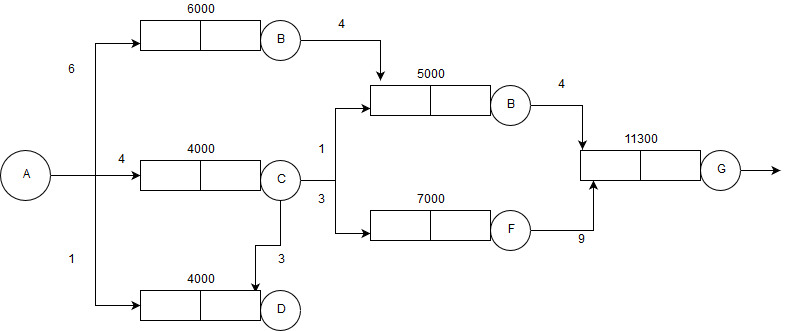
\includegraphics[width=\textwidth]{Images/411.jpg}
\end{figure}
\noindent
Camino incremental: $\mu_1[t,s]=A-B-E-G\fd \alpha_1=4$
\begin{table}[H]
\centering
\begin{tabular}{|c|c|c|c|c|c|c|c|c|c|c|c|}
\hline
\textbf{i} & A & A & A & B & C & C & C & D & E & F & G \\ \hline
\textbf{i} & B & C & D & E & D & E & F & F & G & G & A \\ \hline
\textbf{f} & 4 &   &   & 4 &   &   &   &   & 4 &   &   \\ \hline
\textbf{c} & 6 & 4 & 1 & 4 & 3 & 1 & 3 & 4 & 4 & 9 & 8 \\ \hline
\end{tabular}
\end{table}
    \end{tcolorbox}
    \item Calcular  el  número  máximo  de  transacciones  realizables  en  cada  vuelta  a  la  red  (unidad  de tiempo) de forma que se cumplan las restricciones impuestas en la gestión del SI
    \begin{tcolorbox}[colback=white,colframe=cyan!50!black,fonttitle=\bfseries]

    \end{tcolorbox}
\end{enumerate}

%%%%%%%%%%%%%%%%%%%%
\subsection{Ejercicio 12}

Francisco  Gutiérrez  (Paco)  es  el  nuevo  administrador  informático  de  la  oficina  de  correos  de  Ciudad Universitaria quiere  agilizar el sistema de  gestión de  y para ello ha realizado un estudio que  describe  a continuación:

\begin{itemize}
    \item Existe  un \enquote{punto  de  recepción}  (PR)  general por  donde  acceden todo  tipo  de  tareas.  El  propósito  de este “punto de recepción es clasificar las tareas recibidas y redirigirlas a uno de los tres procesadores A, B o C en función del propósito de cada tarea: envíos nacionales (A), envíos en Europa (B), resto de envíos (C). La  cola  del  PR tiene  una  capacidad  máxima  de  20.000  tareas diarias pero por  cuestiones  técnicas tiene restringida la admisión de tareas en el sistema a 16.000.
    \item El procesador A, que realiza el registro de entrada del paquete, tiene una cola limitada a 5000 tareas. Tras ejecutarse la tarea en este procesador, se produce una solicitud emisión e impresión del recibo en la estación de servicio N (Nacional), cuya capacidad de recepción es de 3.000 tareas.
    \item El procesador B, con funciones similares a A, tiene una cola limitada a 6.000 tareas. Tras el registro del paquete pueden  ocurrir  dos  cosas:  que  la tarea  sea  redirigida  a  la  estación  de  servicio D  donde  se produce  la  impresión  del  recibo o  bien  que  sea  redirigida  a  la  estación  de  servicio E  (inspecciones especiales) donde  se realiza  una  toma  de  datos  adicional.  La capacidad  de  la  cola  de  la D desde  el procesador  B  está  limitada  a  8.000  tareas  mientras  que  la  capacidad de  la  cola  de  la E desde  el procesador B está limitada a 3.000.
    \item Análogamente  a  lo  ocurrido  con  el  procesador  B  ocurre  con  C.  Esta  vez  la  capacidad  de  la  cola  del procesador C es de 6.000 tareas, de ellas las estaciones D y E tienen restringido a un máximo de 4000 la recepción.
    \item La  estación  de  servicio E, inspección  especial,  recoge  tareas  procedentes  del  procesador  B  y  tareas procedentes  del  procesador  C. Tras  la  gestión  de  E, si  no  se  cumplen  ciertos  requisitos,  la tarea  puede ser redirigida a la estación de servicio PR (hasta un máximo de 4.000) o enviada a la estación de servicio D para la impresión del recibo (hasta un máximo de 5.000).
\end{itemize}
Paco ha  sido  informado por  Genaro  (el  anterior  administrador) de cierta  información  útil a tener  en cuenta antes de la reconfiguración de la red:

\begin{itemize}
    \item Se sabe que a la red llega una media de 12.000 tareas diarias, de las cuales el 50\% son de tipo B y de las cuales el 50\% requieren ser inspeccionadas.
    \item El 25\% de las tareas que llegan al sistema son de tipo A.
\end{itemize}

Se  pide  dibujar  la  red  y  encontrar  el  flujo  máximo  (en  media  diaria)  teniendo  en  cuenta  toda  la información.\\
¿Qué alternativas de mejora se pueden plantear teniendo en cuenta estos datos?

\begin{tcolorbox}[colback=white,colframe=cyan!50!black,fonttitle=\bfseries]
\begin{figure}[H]
    \centering
    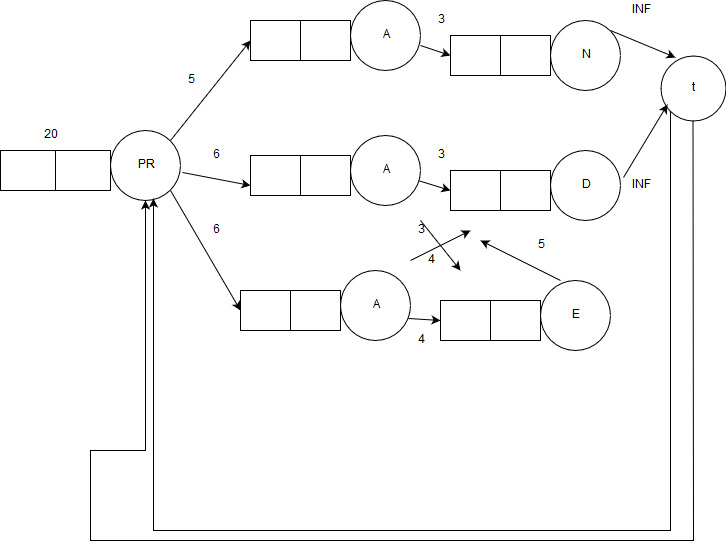
\includegraphics[width=\textwidth]{Images/412.jpg}
\end{figure}
\begin{table}[H]
\centering
\begin{tabular}{|c|c|c|c|c|c|c|c|c|c|c|c|c|c|}
\hline
\textbf{i} & PR & PR & PR & A & B & B & C & C & N   & D   & E & E  & T   \\ \hline
\textbf{j} & A  & B  & C  & N & D & E & D & E & t   & t   & D & PR & PR  \\ \hline
\textbf{f} & 3  & 5  & 6  & 3 & 3 & 3 & 4 & 2 & 3   & 12  & 5 & -  & 15  \\ \hline
\textbf{c} & 5  & 6  & 6  & 3 & 8 & 3 & 4 & 4 & $\inf$ & $\inf$ & 5 & 4  & $\inf$ \\ \hline
\end{tabular}
\end{table}
\[\left.\begin{array}{lllll}
\mu_1=PR-B-E-D-t; \alpha_1=3\fd\alpha_1=\text{minimo flujo máximo del camino}\\
\mu_2=PR-B-D-T; \alpha_2=3\\
\mu_3=PR-A-N-3; \alpha_3=3\\
\mu_4=PR-C-E-D-T; \alpha_4=2\\
\mu_5=PR-C-D-T; \alpha_5=4
\end{array}\right.
\]
15=flujo máximo
\end{tcolorbox}